\begin{explanationbox}
\begin{center}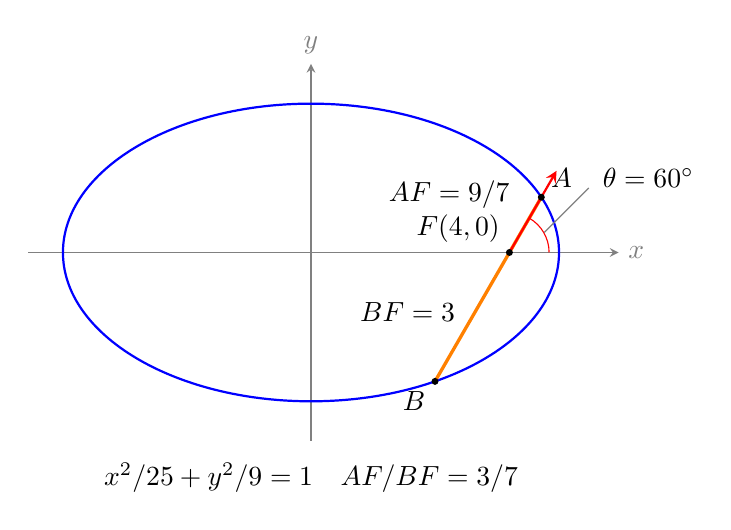
\begin{tikzpicture}[scale=.63,>=stealth]
\draw[->,gray] (-5.7,0)--(6.2,0) node[right] {$x$};
\draw[->,gray] (0,-3.8)--(0,3.8) node[above] {$y$};
\draw[blue,thick] (0,0) ellipse (5 and 3);
\coordinate (F) at (4,0); \coordinate (A) at ({65/14},{9*sqrt(3)/14});
\coordinate (B) at (2.5,{-3*sqrt(3)/2});
\draw[orange,very thick] (B)--(A);
\draw[->,red,thick] (F)--({4+1.9*.5},{1.9*sqrt(3)/2});
\draw[red] (4.8,0) arc (0:60:.8);
\draw[gray] (4.7,.4)--(5.6,1.3);\node at (6.8,1.5) {$\theta=60^\circ$};
\fill (F) circle (2pt) node[above left] {$F(4,0)$};
\fill (A) circle (2pt) node[above right] {$A$};
\fill (B) circle (2pt) node[below left] {$B$};
\node[left] at (3.1,-1.2) {$BF=3$};
\node[above left] at (4.2,.7) {$AF=9/7$};
\node[align=center] at (0,-4.55) {$x^2/25+y^2/9=1$\quad $AF/BF=3/7$};
\end{tikzpicture}
\end{center}
\textbf{先看方向，再记符号。} 图中 $A$ 在从右焦点沿 $60^\circ$ 出发的射线上，
离右端边界较近，所以 $AF<BF$，应有 $AF/BF=3/7$。
当 $\theta=0$ 时，$AF=a-c$、$BF=a+c$，这是检查正负号最快的边界情形。
\par\medskip\noindent
由右准线 $x=a^2/c$ 及第二定义，
$r=e(a^2/c-c-r\cos\theta)$，故 $(a+c\cos\theta)r=b^2$。
反方向将余弦换成 $-\cos\theta$ 即得 $s$。
左焦点的公式需交换余弦符号；双曲线还需区分分支和绝对值，不能机械照搬。
\end{explanationbox}
